\section{Background}
\label{sec:background}

\subsection{RDMA}

Remote Direct Memory Access, or RDMA, is a low-latency, high-throughput networking technology that allows DMA (direct memory access)
read/write requests from a remote machine, without involving the remote CPU. It uses: 1) zero-copy to enable data transfer from application memory
directly to/from NIC, without additional copying into/out of networking stack or operating system buffer; 2) kernel bypass to reduce kernel overhead
and context switch time; and 3) no CPU involvement to eliminate CPU bottleneck on remote machine. RDMA can achieve $\mu$s-level latency and 100/200 Gbps
throughput in modern RDMA-enabled NICs, or RNICs.

\subsection{RoCE and iWARP}

RDMA over Converged Ethernet, or RoCE, is a network protocol that allows RDMA over an Ethernet network.
RDMA was originally designed to run over InfiniBand network and uses InfiniBand-specific headers for routing, etc.
RoCE allows RDMA packets to be transmitted on top of Ethernet layer. In particular, RoCE v1 (or simply RoCE) is an Ethernet link-layer protocol,
as shown on top in \autoref{fig:roce_header_format}. However, at layer 2, it's not routable in Ethernet domain. Thus the standardization body of
RoCE introduced RoCE v2, sometimes refered to as Routing RoCE, or RRoCE in short, an internet layer protocol on top of UDP, to overcome this issue.

It's worth noting that since InfiniBand network is designed to be lossless, using credit-based flow control mechanism, RDMA itself needs a lossless
fabric. This means that RoCE also requires a lossless Ethernet fabric, and this is achieved by using 802.1 Qbb Priority-based Flow Control,
or PFC~\cite{802.1qbb}.

RoCE has comparable raw performance characteristics with RDMA on InfiniBand network. It has made it possible to run RDMA in datacenters
and it's gaining popularity in recent years. Cloud operators like Microsoft Azure has started providing RDMA-capable virtual machines~\cite{news:azure.rdma}.

\begin{figure*}[ht]
    \centering
    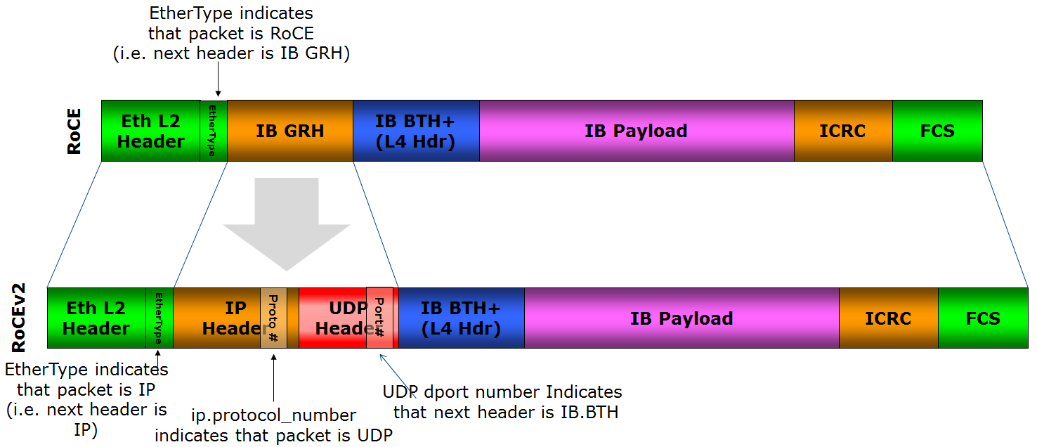
\includegraphics[width=\textwidth]{fig/RoCE_Header_format}
    \caption{RoCE v1 and RoCE v2 packet format}
    \label{fig:roce_header_format}
\end{figure*}

iWARP is an alternative to RoCE for bring RDMA to the Ethernet world. It implements RDMA on top of TCP stack, which is handled by the hardware directly.
Although it doesn't require additional configuration like PFC and run over a generic lossy network,
due to overhead of TCP stack, iWARP performance is much worse than RoCE and thus it hasn't been widely adopted.

\subsection{RDMA Security}

RDMA protocol was originally designed to operate on HPC (High Performance Computing) clusters.
These clusters often are built for a designated purpose, e.g. large-scale physical simulations,
inside a separated and trusted facility. These separated facilities ensure that there is no eavesdropping or compromised on hosts and switches. However, recent adoptions of RDMA in datacenters for cloud refutes the assumption of separation and trustiness. Operating RDMA for cloud environment assumes that malicious users might be able to perform side-channel attacks or even compromise other virtual machines simply by colocation.
Concrete defense measure needs to be addressed to counter the emerging security issues from datacenter-wide RDMA adoptions.

RDMA Applications aim for high speed network links running at typically 40 to 100 Gbps. RDMA transfers data in raw bytes in favor of performance. However, this design decision is only acceptable for HPC clusters but not for VMs in datacenters. Transferring in encrypted data over RDMA should be an important but minimal requirement for RDMA security. The possible security measure of either RoCE and iWARP RDMA can operate on different levels of the protocol stacks, e.g. IPsec or tcpcrypt. However, a TLS-like implementation for RDMA is generally better per end-to-end principle. The inclusion of encryption and authentication should only be on end hosts to prevent laborious change to intermediate switches and routers. DTLS is the counterpart of TLS over UDP, and it works very similarly. Thus we only discuss a TLS-like implementation for TCP in the following paragraphs.

The TLS protocol ensures three properties: secrecy, authenticity, and reliability. Authenticity and reliability are less important in the datacenters. Every computing instances in datacenters can be easily authenticated and we assume the networking in datacenter is reliable as lossless. However, secrecy can be hard to achieve and we will present the difficulties at Sec.~\ref{sec:encrypt}. A TLS implementation has two protocols: Handshake Protocols and Record Protocol. We argue that only Record Protocol is required in datacenters because the handshake protocols can be pre-assigned and updated in a fixed time period for a group of known hosts. In a RoCE v2 packet, there are one 4-byte CRC checksum for Ethernet FCS (Frame Check Sequence) and another 4-byye ICRC for RoCE v2 beyond Ethernet. Using a 4-byte MAC is not enough for any secure MAC algorithm for today's standard. Therefore, we argue that the MAC for TLS-enabled RDMA traffic should be implemented in the payload of InfiniBand.

For RDMA, in a previous work, Security Enhancement in InfiniBand Archetecture~\cite{Lee:2005:SEI:1053727.1054449}, the paper achieves authenticity by embedding an authentication tag in the
header of an IBA packet. \textcolor{red}{TBA}
